\subsection{Command}
\subsubsection{Định nghĩa}
Command là một mẫu thiết kế hành vi (behavioral design pattern) cho phép đóng gói các yêu cầu hoặc hành động vào một đối tượng riêng biệt. Nó chuyển đổi các yêu cầu thành một đối tượng độc lập, cho phép chúng ta thực hiện các yêu cầu, hàng loạt yêu cầu, hoặc hủy yêu cầu một cách linh hoạt.
\subsubsection{Cách sử dụng}
Thông thương, ta hay sử dụng mẫu thiết kế trên trong các trường hợp:
\begin{itemize}
    \item Khi bạn muốn tạo ra một hàng đợi các yêu cầu được thực thi theo thứ tự hoặc lưu trữ lịch sử các yêu cầu.
    \item Khi bạn muốn hỗ trợ hoạt động undo/redo.
    \item Phối hợp nhiều Command với nhau theo thứ tựtự.
\end{itemize}
\subsubsection{Cấu trúc}
\begin{center}
    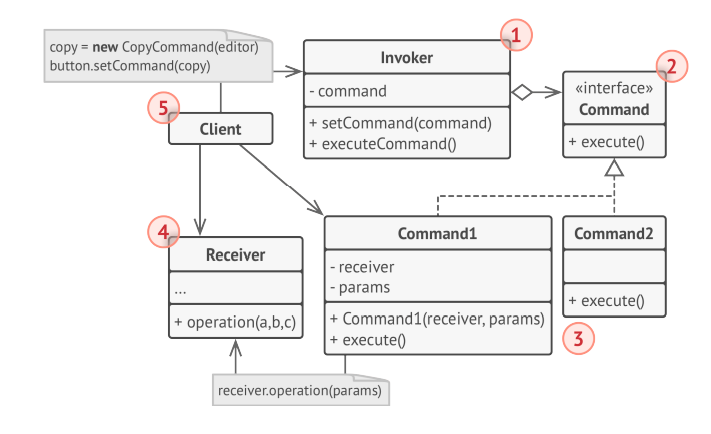
\includegraphics[scale= 0.6]{image/behavioral/command.png}
\end{center}
Các thành phần chính của mẫu:
\begin{itemize}
    \item Command là một interface hoặc abstract class chứa một phương thức thực thi, phương thức trừu tượng.
    \item ConcreteCommand là các subclass của Command định nghĩa operation.
    \item Invoker là một class tiếp nhận từ ConcreteCommand và gọi operation để thực thi.
    \item Receiver là một thành phần thực sử để xử lí cho case. Trong phương thức operation của ConcreteCommand chúng ta sẽ gọi method tương thích trong Receiver.
\end{itemize}
\subsubsection{Ưu điểm và Nhược điểm}
Có các ưu điểm và nhược điểm sau:
Ưu điểm:
\begin{itemize}
    \item Hỗ trợ các tính năng như undo/redo, quản lý lịch sử các yêu cầu.
    \item Giảm sự phụ thuộc giữa người gửi và người nhận yêu cầu.
\end{itemize}
Nhược điểm:
\begin{itemize}
    \item Có thể dẫn đến số lượng lớp lớn nếu có quá nhiều loại yêu cầu.
\end{itemize}

\subsubsection{Code Example}
\begin{itemize}
    \item Có một interface Command và 2 class LightOn và class LightOff được kế thừa.
    \item có class RemoteControl là Invoker có hàm excute để thực thi các lệnh.
\end{itemize}
\begin{lstlisting}
#include <iostream>
#include <string>
#include <vector>

// Command interface
class Command {
public:
    virtual void execute() = 0;
};

// Concrete command 1
class LightOnCommand : public Command {
private:
    std::string light;

public:
    LightOnCommand(const std::string& light) : light(light) {}

    void execute() override {
        std::cout << "Turn on " << light << " light" << std::endl;
    }
};

// Concrete command 2
class LightOffCommand : public Command {
private:
    std::string light;

public:
    LightOffCommand(const std::string& light) : light(light) {}

    void execute() override {
        std::cout << "Turn off " << light << " light" << std::endl;
    }
};

// Invoker
class RemoteControl {
private:
    std::vector<Command*> commands;

public:
    void setCommand(Command* command) {
        commands.push_back(command);
    }

    void executeCommands() {
        for (Command* command : commands) {
            command->execute();
        }
        commands.clear();
    }
};

int main() {
    // Create the invoker
    RemoteControl remote;

    // Create the commands
    Command* cmd1 = new LightOnCommand("Living Room");
    Command* cmd2 = new LightOnCommand("Bedroom");
    Command* cmd3 = new LightOffCommand("Bedroom");
    Command* cmd4 = new LightOffCommand("Living Room");

    // Set the commands
    remote.setCommand(cmd1);
    remote.setCommand(cmd2);
    remote.setCommand(cmd3);
    remote.setCommand(cmd4);

    // Execute the commands
    remote.executeCommands();

    // Clean up
    delete cmd1;
    delete cmd2;
    delete cmd3;
    delete cmd4;

    return 0;
}


\end{lstlisting}
Ở hàm main, ta tạo ra 4 lệnh, add nó vào remote rồi sau đó cho thực hiện cả 4 lệnh đó.\\
\newline
\textbf{Kết quả:}
\begin{lstlisting}
Turn on Living Room light
Turn on Bedroom light
Turn off Bedroom light
Turn off Living Room light
\end{lstlisting}
\subsubsection{Các Pattern liên quan}
\begin{itemize}
    \item CoR: nhận yêu cầu rôi thực hiện lần lượt các commands theo thứ tự.
    \item Mediator: thực hiện thông qua đối tượng gián tiếp.
    \item Observer: định nghĩa mối quan hệ một thay đổi các commands thay đổi theo.
\end{itemize}